\documentclass[conference]{IEEEtran}

\title{
  Course ID2210\\
  Project Report
}

\author{
  \IEEEauthorblockN{Riccardo Reale}
  \IEEEauthorblockA{Peerialism AB\\
    {riccardo.reale@peerialism.com}\\
    \url{https://github.com/riccardoreale/id2210-vt14.git}
  }
  \and
  \IEEEauthorblockN{Giovanni Simoni}
  \IEEEauthorblockA{Peerialism AB\\
    {giovanni.simoni@peerialism.com}\\
    \url{https://github.com/dacav/id2210-vt14.git}
  }
}

\usepackage{xspace}
\usepackage{xcolor}

\usepackage{hyperref}
\hypersetup{
  colorlinks=true,
  linkcolor=black,
  citecolor=black,
  filecolor=black,
  urlcolor=black,
}

\usepackage{braket}
\usepackage{graphicx}
\usepackage{amssymb}
\usepackage{amsmath}
\usepackage{amsthm}
\usepackage{booktabs}
\usepackage{multirow}
\usepackage{paralist}

\usepackage[ruled,vlined,nofillcomment,linesnumbered]{algorithm2e}

\newcommand{\actor}[1]{\textsc{#1}\xspace}
\newcommand{\kword}[1]{\textsc{#1}\xspace}
\newcommand{\component}[1]{\texttt{#1}\xspace}

\newcommand{\us}{\textit{Sparrow}\xspace}
\newcommand{\omni}{\textit{Omniscient}\xspace}

% Actors
\newcommand{\dc}{\actor{Data Center}}
\newcommand{\tmast}{\actor{Task Master}}
\newcommand{\exc}{\actor{Executor}}

% Components
\newcommand{\RmWorker}{\component{RmWorker}}
\newcommand{\ResourceManager}{\component{ResourceManager}}
\newcommand{\FailureDetector}{\component{FailureDetector}}

\newcommand{\treq}{\kword{requisites}}
\newcommand{\Treq}{\kword{Requisites}}
\newcommand{\capable}{\kword{capable}}
\newcommand{\Capable}{\kword{Capable}}



\begin{document}
\maketitle

\section{Architecture design}

  \subsection{Base Sparrow}
  
  The base system was implemented following the suggested design with the addition of 
  two main components initialized by each simulated Peer:
  \begin{enumerate}

  \item A RmWorker component, which abstracts the Resource Manager from task queue
  handling and execution.
  
  \item A FailureDetector component, which detects not responding nodes that are subscribed to be
  monitored. If a monitored node doesn't ACK to alive pings after a certain timeout (3 seconds), the Detector will assume the node to have crashed. For simplicity we assume that on the DataCenter there are no network failures, so if a node is detected as dead, it will stay so.
  
  \end{enumerate}
  
   The required number of CPUs and amount of memory for the execution of a
  task will be referred as \treq. \Treq are allocated by the node executing the
  task (\exc) on behalf of the assigner (\tmast). The allocation time is
  considered as the payload of a task assignment and we assume is not known a priori by a ResourceManager. Therefore the allocation time is used only to simulate the task execution, which consists in allocating the resources (according to \treq), waiting the specified amount of time, and releasing the resources.

  We implemented two different behavioral modes. The first implements
  the best scheduling logic illustrated by the Sparrow paper (Batch + Late Binding), henceforth referred as \us, while the second implements
  an omniscient scheduler for sake of comparison with an optimal assignment
  strategy, henceforth referred as \omni. This is obtained directly in the DataCenter scheduler, which, for each task, will calculate the first node to have the requested resources available, and assign it to be executed directly on that node as soon as possible. This operation is, of course, unrealistic since it make use of both updated information about the task queue on each node, and the allocation time of each task.
  
  The workflow for \us algorithm is the following:
  \begin{enumerate}
  
  \item The task gets issued by the \dc and propagated
        to a \tmast, which is selected as the closest to the task
        identifier within a consistent hash table;

 \item The \tmast probes a number of his neighbours indicating the \treq.
 
 \item The nodes receiving the probe forwards the request to their RmWorker, which put a place-holder in their own waiting queue, and then signal the \tmast that the probe was received.
 
 \item Every time the RmWorker receives a probe, it selects the first task in the waiting queue (which is FIFO) and, if it has enough resources available to execute it, it temporary allocates the \treq resources and request its ResourceManager to ask for a confirmation from the \tmast.
 
 \item When a \tmast receives a request for confirmation from an \exc, it send an Assignment to him with the oldest not-yet-assigned task. The assigned task may differ from the task request sent by the probe, as long as it requires less or equal \treq. In case there are no tasks that can be assigned to the available \exc, it will respond with a Cancel.
 
 \item If an \exc waiting for a confirmation receives an Assignment, its RmWorker de-allocates the temporary blocked resources, and immediately allocates the assigned task and executes it. This is important since the place-holder task may different from the actually assigned one.

 \item If an \exc waiting for a confirmation receives a Cancel instead, its RmWorker simply de-allocates the temporary blocked resources, and executes 4.
 
 \item When a \exc RmWorker completes a task execution, it releases the blocked resources, notifies its ResourceManager and executes 4.
 
  \end{enumerate}
 
 Concerning Fault Tolerance, the ResourceManager subscribes to its FailureDetector each node it probes and check that every probe is received. If a node is detected as dead, the \tmast will restart the probe process for each task that was running on the dead node. Similarly the RmWorker of an \exc subscribes each \tmast. If a \tmast is detected as dead, the RmWorker will cancel all his tasks.
  

  \subsection{Improved Sparrow}
  The improved version of Sparrow consists in four main algorithm modifications:
   \begin{enumerate}

  \item \textbf{Self Assignment }- A ResourceManager receiving a Task from the DataCenter will directly execute it if its RmWorker has enough resources immediately available.
  
  \item \textbf{Probe Propagation} - A ResourceManager receiving a probe can decide to deposit it on its RmWorker or propagating it to another neighbour.  The probe will be locally deposited if its task can be executed immediately or it has been propagated more than a fixed number of time (usually 5).
  
   \item \textbf{Next Hop Selection} - When probing or propagating a probe, the peer selected from the neighbours can be chosen randomly (Random Walks) or in a greedy way (Greedy Search), based on the current knowledge of his resources availability provided by Cyclon We used a SoftMax algorithm with configurable temperature.
  
  \item \textbf{Gradient View} - Instead of using the the neighbors view provided by Cyclon, the RmWorker can use the view provided by Gradient, implemented using a Gradient Ranking function on top of TMan, based on the available node resources. We used a greedy ranking function, while the utility function is very basic and defined as:
\begin{equation}
 U_p(n) = CPU_p(n) - Queue_p(n)
\end{equation}
Where $CPU_p(n)$ means the available CPU of the node \textit{n} according to the value cached by node\textit{ p}, and $Queue_p(n)$ the length of its waiting queue.
   The reason of this choice will be clarified in the Evaluation.
  
  \end{enumerate}

Finally Cyclon gossip period has been configured down to 250ms for  providing fresh samples for Greedy Search and Gradient.

\section{Experimental evaluation}

\subsection{Setup}
To evaluate our improvement over Sparrow we selected two main scenarios:
\begin{itemize}

\item A load scenario where 50 homogeneous nodes (8 cpus and 16GB memory) executes 1000 tasks, each requesting 2 cpus and 2Gb of memory and a fixed execution time of 10 seconds. The load simply determines the inter-arrival time of the tasks, based on the number of total cpu in the DataCenter (the dominant resource) and the processing time.

\item A random scenario (\textbf{A}) which consists in using  a variable number of homogeneous nodes (8 cpus and 16GB memory), executing 500 tasks with different requirements in terms of only cpu (between 1 and 8) and time (between 1 and 30 seconds), which arrive at a rate of half second between each.

\item A random scenario (\textbf{B}) similar to A but tasks have random values of both cpu and memory (between 1 and 8 GB). For this particular scenario we changed the utility function to combine also the available memory.

\item A random scenario (\textbf{C}) similar to A but with heterogeneous nodes resources.

\end{itemize}

Except for scenario \textit{B}, all of them are generated using the CPU as dominant resource, for easily controlling the load and the greedy ranking functions, both for Greedy Search and Gradient.

We added and evaluated the different algorithm improvements adding them to the Sparrow base one to obtain three different configurations: 
\begin{enumerate}
\item \textbf{Random Walk} uses Self Assignment and Probe Propagation, with random Next Hop Selection (Temperature set to 100), giving us Random Walks for each probe. 
\item \textbf{Greedy Search} adds Greedy Next Hop Selection.
\item \textbf{Gradient Search} uses Greedy Next Hop Selection on top of Gradient View.
\end{enumerate}

As main measures we use, as suggested, the average queue time of each task and the 99th percentile. Each result is average over 5 to 10 runs with different seeds.

\subsection{Results in Load Scenario}

Figure \ref{fig:probes} shows the base implementation of Sparrow in the Load scenario, for different number of probes used. The results are consistent with the one presented in the Sparrow work.

Figure \ref{fig:comparison} instead shows the results comparison between the Base Sparrow algorithm (2 probes) and the improved configurations.

\begin{figure}
\begin{center}
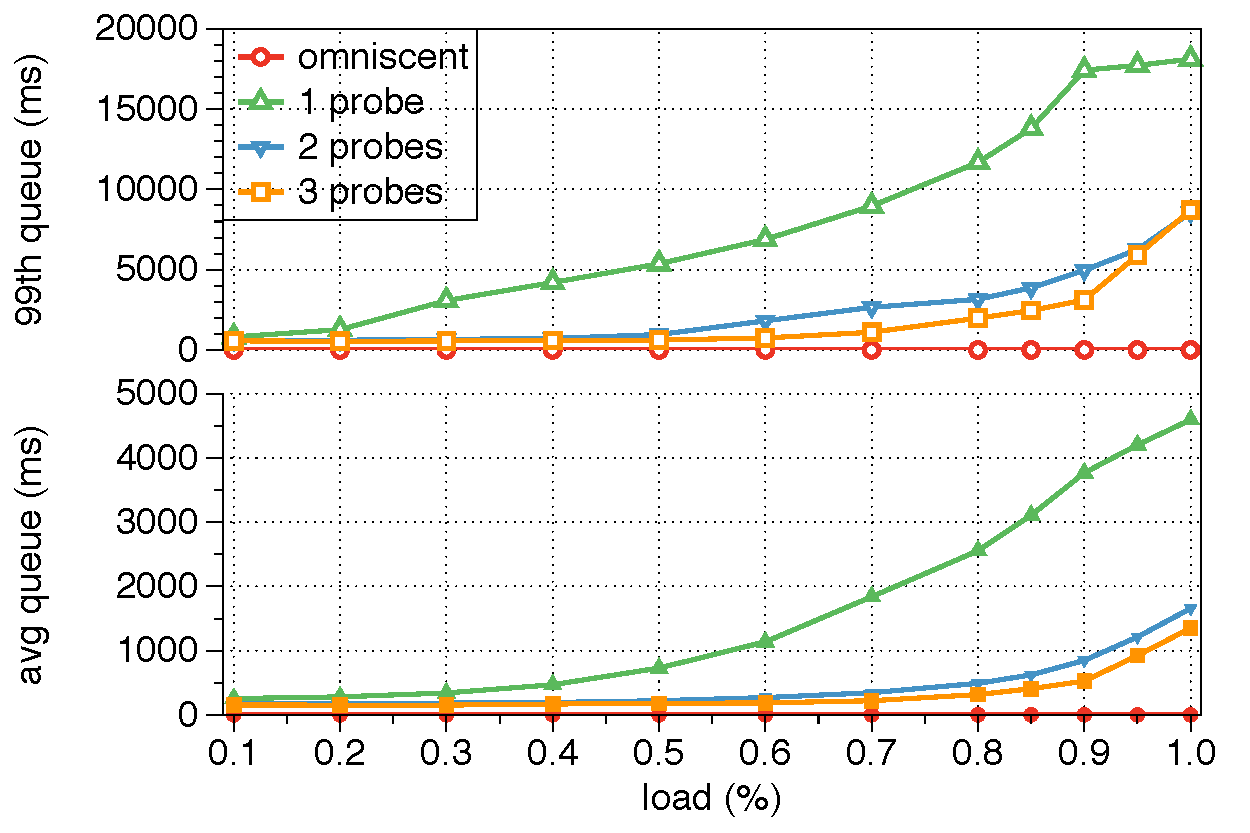
\includegraphics[scale=0.45]{figures/probes_new}
\caption{Base Sparrow algorithm using different load and number of probes}
\label{fig:probes}
\end{center}
\end{figure}

\begin{figure}
\begin{center}
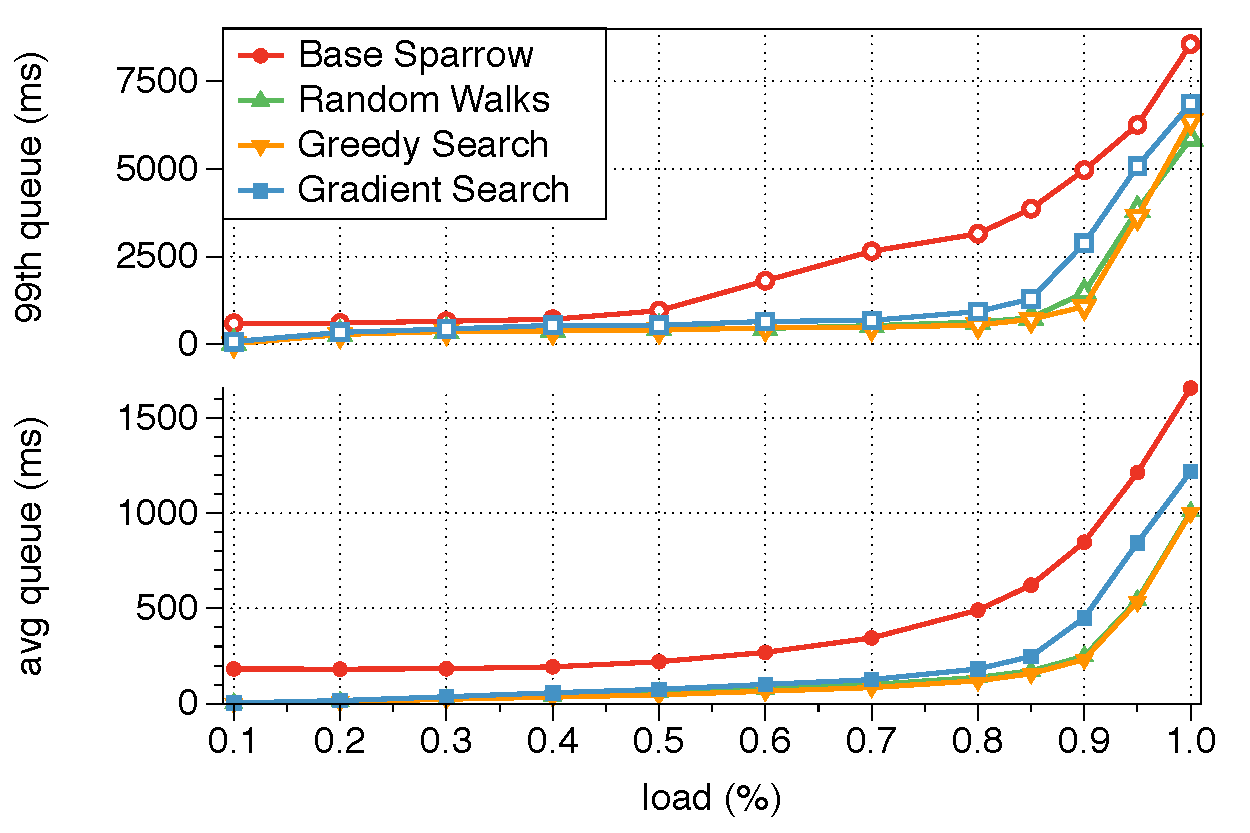
\includegraphics[scale=0.45]{figures/comparison_new}
\caption{Comparison between Base Sparrow Algorithm and its enhancements}
\label{fig:comparison}
\end{center}
\end{figure}

The comparison shows how the Self Assignment decreases the average queue time, since in most cases the task won't be propagated at all but immediately executed on the \tmast.

The Probe Propagation instead decreases dramatically the 99th percentile queue time, especially with loads between 50\% and 85\%, and similarly on all the configurations. Above 85\%, all configurations experience an increase in both average and 99th percentile. 

Using a Greedy Search on top of Random View doesn't improve significantly neither average or 99th percentile.

Finally the last configuration, using Gradient, performs slightly worse than the others. At higher loads probably Cyclon is not fast enough to provide very fresh samples of the neighbour resources, which results on the nodes on top of the gradient to receive an higher amount of probes. 

The Gradient Ranking function is not too useful when the load increases too much since the use of Late Binding provides a poor correlation between waiting queue length and actual load, since any of the place-holder could get a Cancel on confirmation request.

\subsection{Results in Random Scenarios}

\begin{figure}
\begin{center}
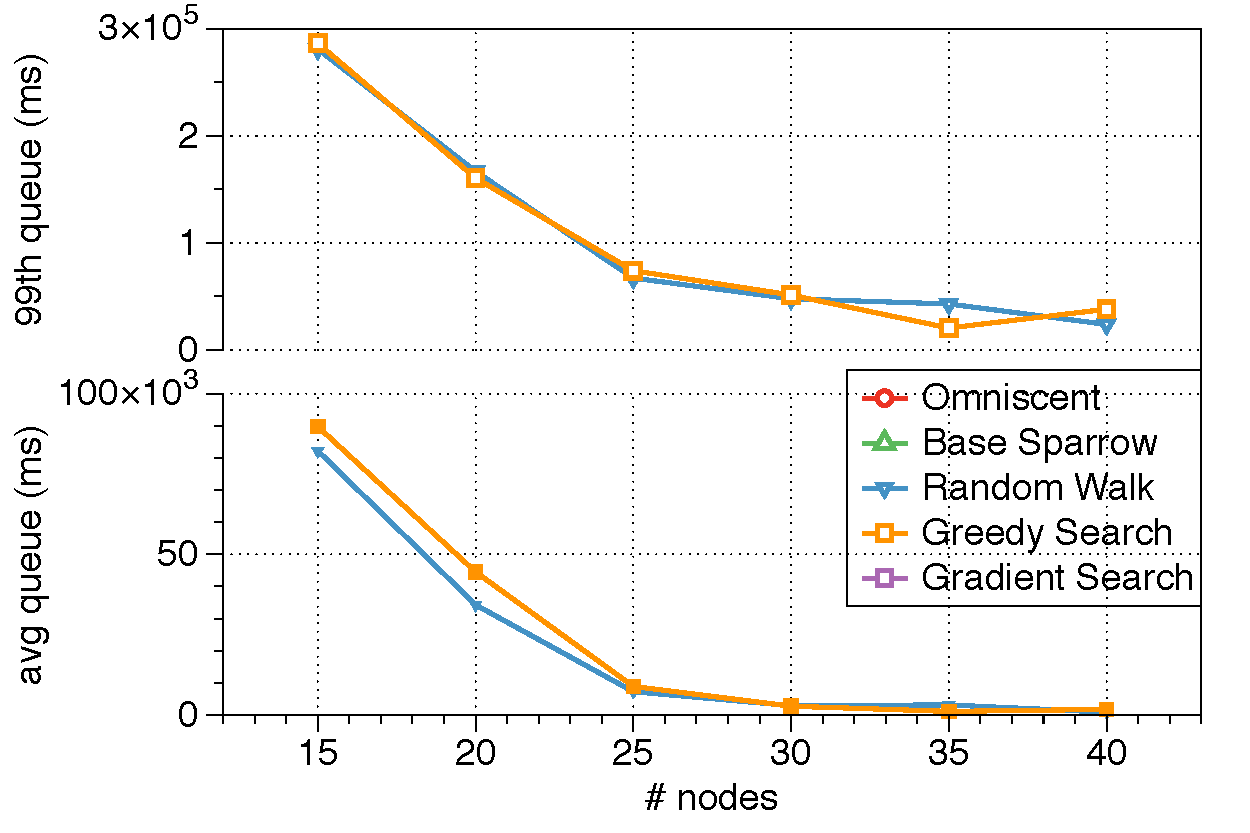
\includegraphics[scale=0.45]{figures/randomA}
\caption{Random Scenario A}
\label{fig:comparison}
\end{center}
\end{figure}

\begin{figure}
\begin{center}
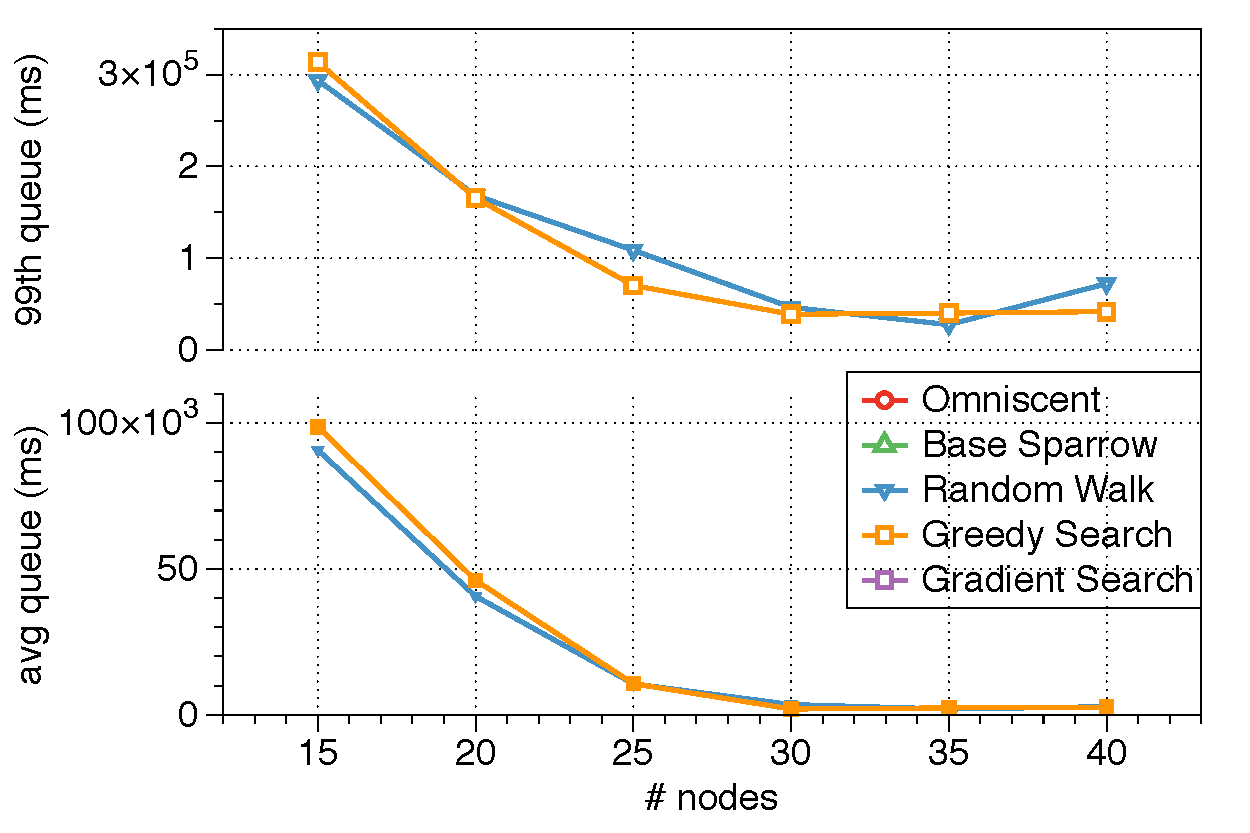
\includegraphics[scale=0.45]{figures/randomB}
\caption{Random Scenario B}
\label{fig:comparison}
\end{center}
\end{figure}

\begin{figure}
\begin{center}
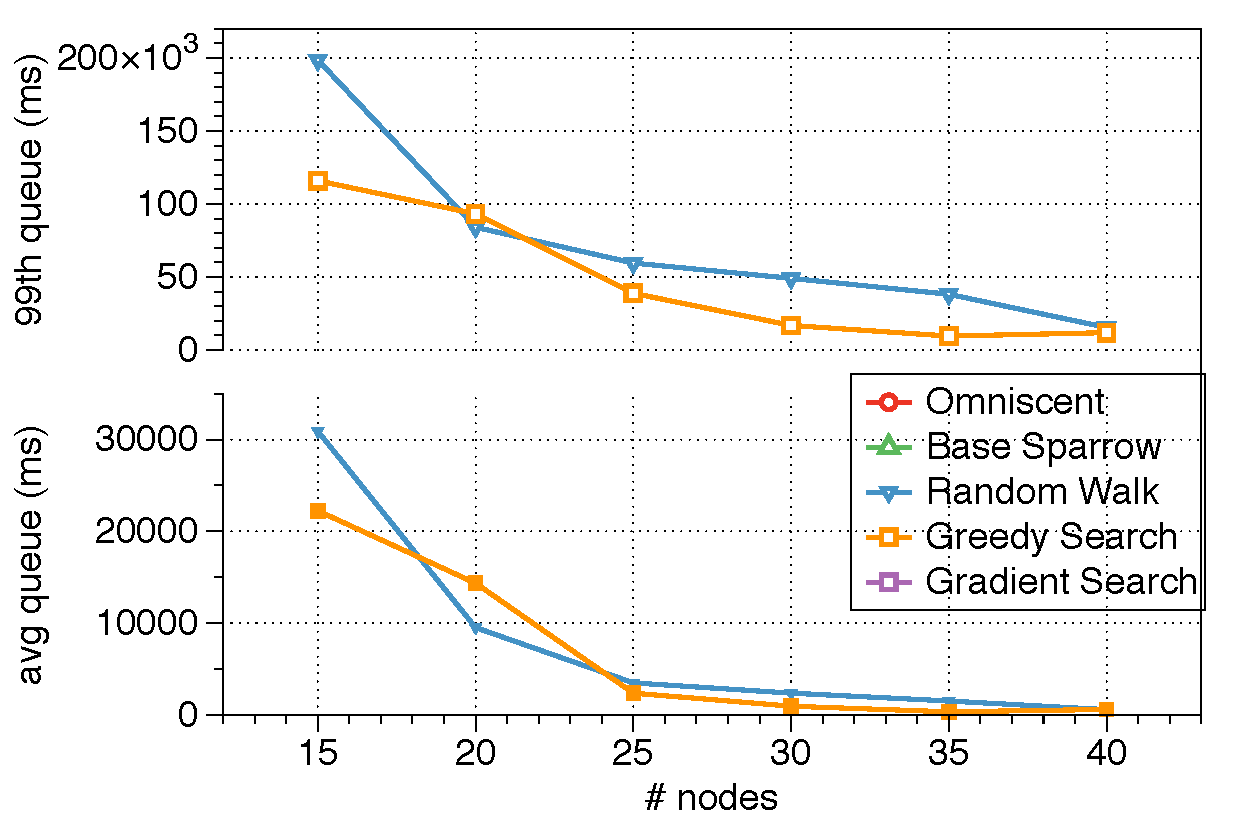
\includegraphics[scale=0.45]{figures/randomC}
\caption{Random Scenario C}
\label{fig:comparison}
\end{center}
\end{figure}

The Random Scenarios show similar trends with the load scenario, with Greedy Search slightly decreasing the Random Walk performances. 
Only in the heterogeneous nodes scenario C the Gradient Search helps decrease the 99th percentile when there are enough resources available (more than 25 nodes).

Therefore, in all scenarios analysed for our implementation, Random Walks, and Greedy Searches gives better result than the base Sparrow algorithm.

The difference between using Random Walks and Greedy Searches are mainly two:
\begin{itemize}
\item the cost of increasing the rate of Cyclon to always provide fresh samples of the utility function
\item the development of a more complex utility function that may take into account multiple resources (more than cpu and memory) and possibly also a better way to estimate queue times (despite Late Binding).
\end{itemize}

.\end{document}
